%%---------------------------------------------------Binary Mixtures-----------------------------------------------------------------------------%%
%%------------------------------------------------------------------------------------------------------------------------------------------------%%

\section{Binary Mixtures}

The bi-level optimization method for parameter estimation, as discussed previously, was successfully applied using the Python programming language. Multi-parameter, constrained optimizers included in the SciPy.Optimize package were used. This method was however found to be very sensitive to initial values and convergence was unreliable. The software would often terminate after a large number of iterations or function evaluations without converging to a feasible solution. This is probably due to the complexity of the unknown overall or underlying mathematical function which is being optimized.\\

In order to overcome this, calculation of binary interaction parameters at various temperatures required manual tweaking of initial parameter guesses for each system, for each model. This is inconvenient and becomes very problematic for cases where the range or order of magnitude of the interaction parameters is not known, for a specific model or mixture. These optimizations may take hours to perform, with no guarantee of convergence.\\

Another problem which was encountered using the bi-level optimization approach was that of parameter scaling. When a model requires that the binary interaction parameters differ greatly, in order to match the experimental measurements, scaling issues prevent the optimization technique from converging properly and reliably.\\

The parameters and phase diagrams for each of the models and each of the binary mixtures in table \ref{BinarySystemsandReferences} where calculated using the pseudo-analytical approach discussed in section \ref{BinaryPAMethodSection}. It was found that this method converged reliably and is relatively insensitive to initial parameter guesses.\\

The pseudo analytical approach does apply a random multi-start approach. This is done in order to ensure convergence to physically significant solutions. However, the solution is readily tested for compliance to certain requirements. This process is automated and therefore requires no manual tweaking. For example, in the case of calculated phase equilibrium compositions, $\sum_{i}^{n} x_{i} = 1$ must apply. Also, the predicted tie-line must have a negative value at $x=0$ and $x=1$. Nevertheless, the pseudo analytical method converged very rapidly, and reliably, in spite of the use of a multi-start approach.\\

For the DWPM the values of $s_{i}$ in equation \ref{DWPMWilsonLike} are chosen as $\nicefrac{1}{2}$. Therefore, the form of the DWPM model used in this investigation reduces to the 3 parameter Wilson model. The software is however programmed to accommodate any values for each $s_{i}$, and the pseudo analytical approach converges equally easily and rapidly for any sensible combination of these parameters. For the NRTL model $\alpha$ is chosen as 0.2, where $\alpha= \alpha_{ij}=\alpha_{ji}$. The pure component constants, $r_{i}$ and $q_{i}$, in the UNIQUAC model are supplied in the Dechema data collection~\cite{Dechema}. The calculated binary interaction parameters for each of the binary mixtures, using the NRTL, UNIQUAC and DWPM models are now presented.\\


%%2-Hexanol-Water

The calculated binary interaction parameters for the mixture 2-Hexanol and Water, for each of the models, at the experimental temperatures is displayed in table \ref{2HexanolWaterTable}. The phase diagram predicted by the DWPM, NRTL and UNIQIAC models, using 10 sets of linearly interpolated parameters, and the original experimentally measured phase compositions are displayed in figures \ref{DWPM2-hexanol-water}, \ref{NRTL2-hexanol-water} and \ref{UNIQUAC2-hexanol-water} respectively.\\

\begin{table}
\begin{tabularx}{\textwidth}{c|cc|cc|cc}
\hline
\textbf{Temperature}&\multicolumn{2}{c|}{\textbf{NRTL}}&\multicolumn{2}{c|}{\textbf{UNIQUAC}}&\multicolumn{2}{c}{\textbf{DWPM}}\\
\hline
\hline
$\left(\mathrm{K}\right)$&$g_{ij}$&$g_{ji}$&$u_{ij}$&$u_{ji}$&$\Lambda_{ij}$&$\Lambda_{ji}$\\
\hline
\textbf{ 293.00 } & -1.011E+02 & 1.788E+03 & 1.780E+02 & 1.659E+02 & 2.423E-03 & 1.159E+00\\
\textbf{ 298.00 } & -1.086E+02 & 1.850E+03 & 1.684E+02 & 1.820E+02 & 2.169E-03 & 1.184E+00\\
\textbf{ 303.00 } & -1.164E+02 & 1.906E+03 & 1.607E+02 & 1.953E+02 & 2.000E-03 & 1.209E+00\\
\hline 
\end{tabularx}\\
\caption{Calculated binary interaction parameters for 2-Hexanol and Water} \label{2HexanolWaterTable}
\end{table}

\begin{figure}[hp]
\centering
\includegraphics[width = 0.85\textwidth]{Results_Parts/BinaryParams/2-hexanol-water/DWPM/PhaseDiagram.eps}
\caption{Calculated phase diagram for 2-Hexanol and Water using the DWPM model} \label{DWPM2-hexanol-water}
\end{figure}

\begin{figure}[hp]
\centering
\includegraphics[width = 0.85\textwidth]{Results_Parts/BinaryParams/2-hexanol-water/NRTL/PhaseDiagram.eps}
\caption{Calculated phase diagram for 2-Hexanol and Water using the NRTL Model} \label{NRTL2-hexanol-water}
\end{figure}	

\begin{figure}[hp]
\centering
\includegraphics[width = 0.85\textwidth]{Results_Parts/BinaryParams/2-hexanol-water/UNIQUAC/PhaseDiagram.eps}
\caption{Calculated phase diagram for 2-Hexanol and Water using the UNIQUAC model} \label{UNIQUAC2-hexanol-water}
\end{figure}	

\clearpage 

For each of the binary mixtures modelled, the $\Delta G_{mix}$ curves, and resulting phase splits, predicted by the NRTL, UNIQUAC and DWPM models are included in the Appendix in section \ref{AppendixGibbsPlotsBinaries}. For each of these plots the change of Gibbs energy on mixing versus composition is determined using the set of calculated interaction parameters, at the relevant temperatures. \\


%%13-Dimethyl Benzene and Water------------------------------------------------------------------------------------------------------------------%%

The calculated parameters for 13-Dimethyl Benzene and Water for each model, at the experimental temperatures is displayed in table \ref{13DimethylBenzeneWaterTable}. As before, the phase diagram predicted by the DWPM, NRTL and UNIQIAC models, using 10 sets of linearly interpolated parameters, and the original experimentally measured phase compositions are displayed in figures \ref{DWPM13DimethylBenzeneWater}, \ref{NRTL13DimethylBenzeneWater} and \ref{UNIQUAC13DimethylBenzeneWater} respectively.\\

\begin{table}
\begin{tabularx}{\textwidth}{c|cc|cc|cc}
\hline
\textbf{Temperature}&\multicolumn{2}{c|}{\textbf{NRTL}}&\multicolumn{2}{c|}{\textbf{UNIQUAC}}&\multicolumn{2}{c}{\textbf{DWPM}}\\
\hline
\hline 
$\left(\mathrm{K}\right)$&$g_{ij}$&$g_{ji}$&$u_{ij}$&$u_{ji}$&$\Lambda_{ij}$&$\Lambda_{ji}$\\
\hline
\textbf{ 292.85 } & 1.386E+03 & 2.541E+03 & 1.000E+03 & 3.371E+02 & 1.579E-04 & 1.352E-02\\
\textbf{ 312.85 } & 1.265E+03 & 2.626E+03 & 9.282E+02 & 3.376E+02 & 1.987E-04 & 2.588E-02\\
\textbf{ 342.85 } & 1.033E+03 & 2.741E+03 & 7.842E+02 & 3.337E+02 & 2.808E-04 & 6.865E-02\\
\hline
\end{tabularx}\\
\caption{Calculated binary interaction parameters for 13-Dimethyl Benzene and Water} \label{13DimethylBenzeneWaterTable}
\end{table}

\begin{figure}[hp]
\centering
\includegraphics[width = 0.85\textwidth]{Results_Parts/BinaryParams/13-dimethylbenzene-water/DWPM/PhaseDiagram.eps}
\caption{Calculated phase diagram for 13-Dimethyl Benzene and Water using the DWPM model} \label{DWPM13DimethylBenzeneWater}
\end{figure}

\begin{figure}[hp]
\centering
\includegraphics[width = 0.85\textwidth]{Results_Parts/BinaryParams/13-dimethylbenzene-water/NRTL/PhaseDiagram.eps}
\caption{Calculated phase diagram for 13-Dimethyl Benzene and Water using the NRTL Model} \label{NRTL13DimethylBenzeneWater}
\end{figure}	

\begin{figure}[hp]
\centering
\includegraphics[width = 0.85\textwidth]{Results_Parts/BinaryParams/13-dimethylbenzene-water/UNIQUAC/PhaseDiagram.eps}
\caption{Calculated phase diagram for 13-Dimethyl Benzene and Water using the UNIQUAC model} \label{UNIQUAC13DimethylBenzeneWater}
\end{figure}	

\clearpage

%% Aniline and Water-----------------------------------------------------------------------------------------------------------------------------%%

The results for the mixture Aniline and Water for each model, at the experimental temperatures are displayed in table \ref{AnilineWaterTable}. The calculated phase diagrams using the DWPM, NRTL and UNIQIAC models are presented in figures \ref{DWPManiline-water}, \ref{NRTLaniline-water} and \ref{UNIQUACaniline-water} respectively. The binary interaction parameters were again linearly interpolated at 9 equally spaced intervals for the construction of the phase diagrams. 

\begin{table}
\begin{tabularx}{\textwidth}{c|cc|cc|cc}
\hline
\textbf{Temperature}&\multicolumn{2}{c|}{\textbf{NRTL}}&\multicolumn{2}{c|}{\textbf{UNIQUAC}}&\multicolumn{2}{c}{\textbf{DWPM}}\\
\hline
\hline 
$\left(\mathrm{K}\right)$&$g_{ij}$&$g_{ji}$&$u_{ij}$&$u_{ji}$&$\Lambda_{ij}$&$\Lambda_{ji}$\\
\hline
\textbf{ 281.60 } & 1.944E+01 & 1.384E+03 & 1.576E+02 & 1.056E+02 & 7.805E-03 & 7.746E-01\\
\textbf{ 298.40 } & -4.970E+01 & 1.510E+03 & 9.818E+01 & 1.465E+02 & 6.999E-03 & 9.409E-01\\
\textbf{ 321.00 } & -4.920E+01 & 1.582E+03 & 1.283E+02 & 1.290E+02 & 7.994E-03 & 9.237E-01\\
\textbf{ 339.30 } & -9.394E+01 & 1.655E+03 & 1.166E+02 & 1.281E+02 & 8.663E-03 & 1.011E+00\\
\textbf{ 369.70 } & -2.231E+02 & 1.800E+03 & 5.003E+01 & 1.518E+02 & 9.514E-03 & 1.273E+00\\
\hline
\end{tabularx}\\
\caption{Calculated binary interaction parameters for Aniline and Water} \label{AnilineWaterTable}
\end{table}

\begin{figure}[hp]
\centering
\includegraphics[width = 0.85\textwidth]{Results_Parts/BinaryParams/aniline-water/DWPM/PhaseDiagram.eps}
\caption{Calculated phase diagram for Aniline and Water using the DWPM model} \label{DWPManiline-water}
\end{figure}

\begin{figure}[hp]
\centering
\includegraphics[width = 0.85\textwidth]{Results_Parts/BinaryParams/aniline-water/NRTL/PhaseDiagram.eps}
\caption{Calculated phase diagram for Aniline and Water using the NRTL Model} \label{NRTLaniline-water}
\end{figure}	

\begin{figure}[hp]
\centering
\includegraphics[width = 0.85\textwidth]{Results_Parts/BinaryParams/aniline-water/UNIQUAC/PhaseDiagram.eps}
\caption{Calculated phase diagram for Aniline and Water using the UNIQUAC model} \label{UNIQUACaniline-water}
\end{figure}	

\clearpage

%% Diethylene Glycol and 12-Dimethyl Benzene-----------------------------------------------------------------------------------------------------%%

The calculated binary interaction parameters for  Diethylene Glycol and 12-Dimethyl Benzene is displayed in table \ref{DiethyleneGlycoland12-DimethylBenzeneTable}. The phase diagram predicted by the DWPM, NRTL and UNIQIAC models, using 10 sets of linearly interpolated parameters, and the original experimentally measured phase compositions are displayed in figures \ref{DWPMdiethyleneglycol-12-dimethylbenzene}, \ref{NRTLdiethyleneglycol-12-dimethylbenzene} and \ref{UNIQUACdiethyleneglycol-12-dimethylbenzene} respectively.\\

\begin{table}
\begin{tabularx}{\textwidth}{c|cc|cc|cc}
\hline
\textbf{Temperature}&\multicolumn{2}{c|}{\textbf{NRTL}}&\multicolumn{2}{c|}{\textbf{UNIQUAC}}&\multicolumn{2}{c}{\textbf{DWPM}}\\
\hline
\hline 
$\left(\mathrm{K}\right)$&$g_{ij}$&$g_{ji}$&$u_{ij}$&$u_{ji}$&$\Lambda_{ij}$&$\Lambda_{ji}$\\
\hline
\textbf{ 313.30 } & 2.424E+02 & 1.463E+03 & -3.846E+01 & 4.915E+02 & 9.234E-03 & 4.125E-01\\
\textbf{ 332.80 } & 1.771E+02 & 1.262E+03 & -4.489E+01 & 4.285E+02 & 2.315E-02 & 4.917E-01\\
\textbf{ 353.80 } & 1.817E+02 & 1.252E+03 & -4.372E+01 & 4.243E+02 & 3.003E-02 & 4.967E-01\\
\textbf{ 363.00 } & 2.279E+02 & 1.064E+03 & -1.779E+01 & 3.525E+02 & 5.441E-02 & 4.460E-01\\
\textbf{ 393.00 } & 1.641E+02 & 1.038E+03 & -3.698E+01 & 3.511E+02 & 7.420E-02 & 5.422E-01\\
\hline
\end{tabularx}\\
\caption{Calculated binary interaction parameters for Diethylene Glycol and 12-Dimethyl Benzene} \label{DiethyleneGlycoland12-DimethylBenzeneTable}
\end{table}

\begin{figure}[hp]
\centering
\includegraphics[width = 0.85\textwidth]{Results_Parts/BinaryParams/diethyleneglycol-12-dimethylbenzene/DWPM/PhaseDiagram.eps}
\caption{Calculated phase diagram for Diethylene Glycol and 12-Dimethyl Benzene using the DWPM model} \label{DWPMdiethyleneglycol-12-dimethylbenzene}
\end{figure}\

\begin{figure}[hp]
\centering
\includegraphics[width = 0.85\textwidth]{Results_Parts/BinaryParams/diethyleneglycol-12-dimethylbenzene/NRTL/PhaseDiagram.eps}
\caption{Calculated phase diagram for Diethylene Glycol and 12-Dimethyl Benzene using the NRTL model} \label{NRTLdiethyleneglycol-12-dimethylbenzene}
\end{figure}\	

\begin{figure}[hp]
\centering
\includegraphics[width = 0.85\textwidth]{Results_Parts/BinaryParams/diethyleneglycol-12-dimethylbenzene/UNIQUAC/PhaseDiagram.eps}
\caption{Calculated phase diagram for Diethylene Glycol and 12-Dimethyl Benzene using the UNIQUAC model} \label{UNIQUACdiethyleneglycol-12-dimethylbenzene}
\end{figure}\	

\clearpage

%%Dipropyl Ether and Water----------------------------------------------------------------------------------------------------------------------%%

The calculated binary interaction parameters for  Dipropyl Ether and Water is displayed in table \ref{dipropylether-waterTable}. The phase diagram predicted by the DWPM, NRTL and UNIQIAC models, using 10 sets of linearly interpolated parameters, and the original experimentally measured phase compositions are displayed in figures \ref{DWPMdipropylether-water}, \ref{NRTLdipropylether-water} and \ref{UNIQUACdipropylether-water} respectively.\\

\begin{table}
\begin{tabularx}{\textwidth}{c|cc|cc|cc}
\hline
\textbf{Temperature}&\multicolumn{2}{c|}{\textbf{NRTL}}&\multicolumn{2}{c|}{\textbf{UNIQUAC}}&\multicolumn{2}{c}{\textbf{DWPM}}\\
\hline
\hline 
$\left(\mathrm{K}\right)$&$g_{ij}$&$g_{ji}$&$u_{ij}$&$u_{ji}$&$\Lambda_{ij}$&$\Lambda_{ji}$\\
\hline
\textbf{ 273.00 } & 6.092E+02 & 1.334E+03 & 7.281E+02 & 6.859E+01 & 6.793E-03 & 1.029E-01\\
\textbf{ 283.00 } & 6.872E+02 & 1.474E+03 & 7.732E+02 & 9.605E+01 & 4.888E-03 & 8.704E-02\\
\textbf{ 288.00 } & 6.827E+02 & 1.548E+03 & 7.646E+02 & 1.095E+02 & 4.128E-03 & 9.360E-02\\
\textbf{ 293.00 } & 6.418E+02 & 1.627E+03 & 7.289E+02 & 1.234E+02 & 3.447E-03 & 1.138E-01\\
\textbf{ 298.00 } & 6.090E+02 & 1.699E+03 & 7.003E+02 & 1.359E+02 & 2.969E-03 & 1.336E-01\\
\hline
\end{tabularx}\\
\caption{Calculated binary interaction parameters for Dipropyl Ether and Water} \label{dipropylether-waterTable}
\end{table}

\begin{figure}[hp]
\centering
\includegraphics[width = 0.85\textwidth]{Results_Parts/BinaryParams/dipropylether-water/DWPM/PhaseDiagram.eps}
\caption{Calculated phase diagram for Dipropyl Ether and Water using the DWPM model} \label{DWPMdipropylether-water}
\end{figure}

\begin{figure}[hp]
\centering
\includegraphics[width = 0.85\textwidth]{Results_Parts/BinaryParams/dipropylether-water/NRTL/PhaseDiagram.eps}
\caption{Calculated phase diagram for Dipropyl Ether and Water using the NRTL model} \label{NRTLdipropylether-water}
\end{figure}	

\begin{figure}[hp]
\centering
\includegraphics[width = 0.85\textwidth]{Results_Parts/BinaryParams/dipropylether-water/UNIQUAC/PhaseDiagram.eps}
\caption{Calculated phase diagram for Dipropyl Ether and Water using the UNIQUAC model} \label{UNIQUACdipropylether-water}
\end{figure}	


\clearpage

%% Ethyl Ester Acetic Acid and Water------------------------------------------------------------------------------------------------------------%%

The calculated binary interaction parameters for Ethyl Ester Acetic Acid and Water is displayed in table \ref{ethylesteraceticacid-waterTable}. The phase diagram predicted by the DWPM, NRTL and UNIQIAC models, using 10 sets of linearly interpolated parameters, and the original experimentally measured phase compositions are displayed in figures \ref{DWPMethylesteraceticacid-water}, \ref{NRTLethylesteraceticacid-water} and \ref{UNIQUACethylesteraceticacid-water} respectively.\\

\begin{table}
\begin{tabularx}{\textwidth}{c|cc|cc|cc}
\hline
\textbf{Temperature}&\multicolumn{2}{c|}{\textbf{NRTL}}&\multicolumn{2}{c|}{\textbf{UNIQUAC}}&\multicolumn{2}{c}{\textbf{DWPM}}\\
\hline
\hline 
$\left(\mathrm{K}\right)$&$g_{ij}$&$g_{ji}$&$u_{ij}$&$u_{ji}$&$\Lambda_{ij}$&$\Lambda_{ji}$\\
\hline
\textbf{ 273.00 } & 2.689E+02 & 8.719E+02 & 4.731E+02 & 2.994E+01 & 4.046E-02 & 3.195E-01\\
\textbf{ 278.00 } & 2.513E+02 & 9.204E+02 & 4.598E+02 & 3.930E+01 & 3.626E-02 & 3.453E-01\\
\textbf{ 283.00 } & 2.337E+02 & 9.685E+02 & 4.465E+02 & 4.882E+01 & 3.266E-02 & 3.721E-01\\
\textbf{ 288.00 } & 2.163E+02 & 1.016E+03 & 4.332E+02 & 5.844E+01 & 2.957E-02 & 3.997E-01\\
\textbf{ 293.00 } & 1.990E+02 & 1.063E+03 & 4.199E+02 & 6.815E+01 & 2.692E-02 & 4.281E-01\\
\textbf{ 298.00 } & 1.809E+02 & 1.110E+03 & 4.059E+02 & 7.808E+01 & 2.460E-02 & 4.586E-01\\
\textbf{ 303.00 } & 1.621E+02 & 1.157E+03 & 3.914E+02 & 8.824E+01 & 2.255E-02 & 4.908E-01\\
\textbf{ 308.00 } & 1.434E+02 & 1.203E+03 & 3.771E+02 & 9.841E+01 & 2.078E-02 & 5.239E-01\\
\textbf{ 313.00 } & 1.241E+02 & 1.250E+03 & 3.623E+02 & 1.088E+02 & 1.922E-02 & 5.587E-01\\
\hline
\end{tabularx}\\
\caption{Calculated binary interaction parameters for Ethyl Ester Acetic Acid and Water} \label{ethylesteraceticacid-waterTable}
\end{table}


\begin{figure}[hp]
\centering
\includegraphics[width = 0.85\textwidth]{Results_Parts/BinaryParams/ethylesteraceticacid-water/DWPM/PhaseDiagram.eps}
\caption{Calculated phase diagram for Ethyl Ester Acetic Acid and Water using the DWPM model} \label{DWPMethylesteraceticacid-water}
\end{figure}

\begin{figure}[hp]
\centering
\includegraphics[width = 0.85\textwidth]{Results_Parts/BinaryParams/ethylesteraceticacid-water/NRTL/PhaseDiagram.eps}
\caption{Calculated phase diagram for Ethyl Ester Acetic Acid and Water using the NRTL model} \label{NRTLethylesteraceticacid-water}
\end{figure}	

\begin{figure}[hp]
\centering
\includegraphics[width = 0.85\textwidth]{Results_Parts/BinaryParams/ethylesteraceticacid-water/UNIQUAC/PhaseDiagram.eps}
\caption{Calculated phase diagram for Ethyl Ester Acetic Acid and Water using the UNIQUAC model} \label{UNIQUACethylesteraceticacid-water}
\end{figure}	

\clearpage


%%Methanol and Heptane--------------------------------------------------------------------------------------------------------------------------%%

The calculated binary interaction parameters for Methanol and Heptane is displayed in table \ref{methanol-heptaneTable}. The phase diagram predicted by the DWPM, NRTL and UNIQIAC models, using 10 sets of linearly interpolated parameters, and the original experimentally measured phase compositions are displayed in figures \ref{DWPMmethanol-heptane}, \ref{NRTLmethanol-heptane} and \ref{UNIQUACmethanol-heptane} respectively.\\


\begin{table}
\begin{tabularx}{\textwidth}{c|cc|cc|cc}
\hline
\textbf{Temperature}&\multicolumn{2}{c|}{\textbf{NRTL}}&\multicolumn{2}{c|}{\textbf{UNIQUAC}}&\multicolumn{2}{c}{\textbf{DWPM}}\\
\hline
\hline 
$\left(\mathrm{K}\right)$&$g_{ij}$&$g_{ji}$&$u_{ij}$&$u_{ji}$&$\Lambda_{ij}$&$\Lambda_{ji}$\\
\hline
\textbf{ 291.00 } & 5.169E+02 & 4.396E+02 & 5.751E+00 & 6.875E+02 & 2.004E-01 & 1.574E-01\\
\textbf{ 303.00 } & 5.494E+02 & 3.490E+02 & 2.189E+00 & 6.460E+02 & 2.828E-01 & 1.559E-01\\
\textbf{ 313.00 } & 5.870E+02 & 2.647E+02 & 5.246E-01 & 6.071E+02 & 3.772E-01 & 1.506E-01\\
\textbf{ 323.00 } & 6.263E+02 & 1.640E+02 & -2.095E+00 & 5.588E+02 & 5.146E-01 & 1.461E-01\\
\hline
\end{tabularx}\\
\caption{Calculated binary interaction parameters for Methanol and Heptane} \label{methanol-heptaneTable}
\end{table}

\begin{figure}[hp]
\centering
\includegraphics[width = 0.85\textwidth]{Results_Parts/BinaryParams/methanol-heptane/DWPM/PhaseDiagram.eps}
\caption{Calculated phase diagram for Methanol and Heptane using the DWPM model} \label{DWPMmethanol-heptane}
\end{figure}

\begin{figure}[hp]
\centering
\includegraphics[width = 0.85\textwidth]{Results_Parts/BinaryParams/methanol-heptane/NRTL/PhaseDiagram.eps}
\caption{Calculated phase diagram for Methanol and Heptane using the NRTL model} \label{NRTLmethanol-heptane}
\end{figure}	

\begin{figure}[hp]
\centering
\includegraphics[width = 0.85\textwidth]{Results_Parts/BinaryParams/methanol-heptane/UNIQUAC/PhaseDiagram.eps}
\caption{Calculated phase diagram for Methanol and Heptane using the UNIQUAC model} \label{UNIQUACmethanol-heptane}
\end{figure}	

\clearpage

%%Methanol and Hexane-------------------------------------------------------------------------------------------------------------------------%

The calculated binary interaction parameters for Methanol and Hexane is displayed in table \ref{methanol-hexaneTable}. The phase diagram predicted by the DWPM, NRTL and UNIQIAC models, using 10 sets of linearly interpolated parameters, and the original experimentally measured phase compositions are displayed in figures \ref{DWPMmethanol-hexane}, \ref{NRTLmethanol-hexane} and \ref{UNIQUACmethanol-hexane} respectively.\\

\begin{table}
\begin{tabularx}{\textwidth}{c|cc|cc|cc}
\hline
\textbf{Temperature}&\multicolumn{2}{c|}{\textbf{NRTL}}&\multicolumn{2}{c|}{\textbf{UNIQUAC}}&\multicolumn{2}{c}{\textbf{DWPM}}\\
\hline
\hline 
$\left(\mathrm{K}\right)$&$g_{ij}$&$g_{ji}$&$u_{ij}$&$u_{ji}$&$\Lambda_{ij}$&$\Lambda_{ji}$\\
\hline
\textbf{ 255.20 } & 4.318E+02 & 5.363E+02 & 2.704E+01 & 6.656E+02 & 1.131E-01 & 1.652E-01\\
\textbf{ 278.00 } & 4.197E+02 & 4.631E+02 & 1.110E+01 & 6.413E+02 & 1.752E-01 & 2.019E-01\\
\textbf{ 298.00 } & 4.405E+02 & 3.443E+02 & 9.253E-02 & 5.877E+02 & 2.881E-01 & 2.160E-01\\
\hline
\end{tabularx}\\
\caption{Calculated binary interaction parameters for Methanol and Hexane} \label{methanol-hexaneTable}
\end{table}

\begin{figure}[hp]
\centering
\includegraphics[width = 0.85\textwidth]{Results_Parts/BinaryParams/methanol-hexane/DWPM/PhaseDiagram.eps}
\caption{Calculated phase diagram for Methanol and Heptane using the DWPM model} \label{DWPMmethanol-hexane}
\end{figure}

\begin{figure}[hp]
\centering
\includegraphics[width = 0.85\textwidth]{Results_Parts/BinaryParams/methanol-hexane/NRTL/PhaseDiagram.eps}
\caption{Calculated phase diagram for Methanol and Hexane using the NRTL model} \label{NRTLmethanol-hexane}
\end{figure}	

\begin{figure}[hp]
\centering
\includegraphics[width = 0.85\textwidth]{Results_Parts/BinaryParams/methanol-hexane/UNIQUAC/PhaseDiagram.eps}
\caption{Calculated phase diagram for Methanol and Hexane using the UNIQUAC model} \label{UNIQUACmethanol-hexane}
\end{figure}	

